\documentclass[aps,twocolumn,pra,notitlepage,]{revtex4-2}
%twocolumn, 
\usepackage{amsmath,amssymb}
\usepackage{dsfont}
\usepackage{graphicx}
\usepackage{physics}
\usepackage{hyperref}
\usepackage{mathtools}
\usepackage{cancel}
\usepackage{bbold}
\usepackage{bm}
\usepackage{color} 
\usepackage[dvipsnames]{xcolor}
\usepackage[T1]{fontenc}

\usepackage{tcolorbox}

\usepackage{soul}
\newcommand{\ttau}{\boldsymbol{\tau}}


\newcommand{\kb}{k_\text{B}}
\newcommand{\ud}{\uparrow\downarrow}
\newcommand{\zem}{\omega}
\newcommand{\tauinf}{\tau}
\newcommand{\dzem}{\delta\zem}
\newcommand{\azem}{\overline\zem}
\newcommand{\tun}{t_{c}}
\newcommand{\te}{\tau}  % what to use for time? t or \tau?
\newcommand{\cnoise}{\xi}
\newcommand{\cnoisee}{\xi_\epsilon}
\newcommand{\cnoiset}{\xi_t}
\newcommand{\mnoise}{\eta}
\newcommand{\eadiab}{A}
\newcommand{\kv}{\mathbf k}
\newcommand{\vecsig}{\boldsymbol{\sigma}}
\newcommand{\JK}[1]{\textcolor{blue}{\small JK: #1}}
\newcommand{\LC}[1]{\textcolor{magenta}{#1}}
\newcommand{\adiab}[1]{{\tilde #1}}

\usepackage{ulem} % Crossing out with \sout{...}                      
\newcommand{\out}[1]{\textcolor{blue}{\sout{#1}}}
\newcommand{\add}[1]{\textcolor{red}{#1}}  


\begin{document}
\newcounter{theo}
\author{Jan A. Krzywda}\email{j.a.krzywda@liacs.leidenuniv.nl}
\author{Evert van Nieuwenburg}
\affiliation{$\langle aQa^L
\rangle$ Applied Quantum Algorithms, Lorentz Institute and Leiden Institute of Advanced Computer Science,
Leiden University, P.O. Box 9506, 2300 RA Leiden, The Netherlands}

\title{TITLE} 


\begin{abstract}

\end{abstract}
\maketitle

\section{Introduction}
In most quantum hardware, interactions between qubits and their environment lead to fluctuations in Hamiltonian parameters, degrading gate fidelity [] and causing decoherence []. While environmental noise is often modeled with a Markovian approach [], which assumes no temporal correlations between experimental runs [], temporally correlated noise dominates in many solid-state qubits []. In this case, the decoherence can be modeled by a classical stochastic process in the qubit Hamiltonian [], which evolves slowly relative to qubit operation times. As a result, the relatively short \( T_2^* \) decoherence timescale [] is limited by the lack of knowledge of Hamiltonian parameters, and hence could strongly benefit from suitable feedback control protocols [].

The presence of correlated noise may require mitigation techniques beyond the standard Quantum Error Correction (QEC) [] and Quantum Error Mitigation (QEM) [] strategies. The most popular methods are Dynamical Decoupling and Pauli Twirling, which require additional control pulses []. An alternative approach involves Bayesian tracking of Hamiltonian parameters [], which has recently been demonstrated in spin qubits []. This allows for feedback-loop control of time-varying parameters but introduces an overhead due to additional single shots needed for estimation.

Unlike in well-established methods for estimating static fields [], online tracking introduces the risk of parameter drift during the estimation period []. This can be naturally mitigated by improving estimation speed. One way of decreasing the number of estimation shots is a physics-informed approach [], in which knowledge about the field is propagated between estimation rounds []. However, this method requires statistical knowledge about the noise, necessitating resource-intensive methods like noise spectroscopy [] or gate-set tomography []. Moreover, the method assumes the Markovian property of the stochastic process, which, for instance, does not hold for 1/f charge noise dominant in solid-state qubits [].

Another method to balance estimation accuracy and speed is the adaptive approach [], facilitated by the fast operation of FPGA-based qubit control []. This approach has reduced the number of shots by adaptively choosing the next probing time based on the current knowledge about the field []. So far, however, only greedy and heuristic adaptive methods have been pursued [], due to the difficulty of finding an optimal scheme that accounts for multiple estimation shots.

The task of finding an adaptive policy to achieve the goal in an unknown environment is a typical setup for Reinforcement Learning (RL) []. In this technique, the agent discovers the policy that maximizes the reward signal through interaction with the environment. So far, RL techniques have been used to improve qubit initialization [], qubit tuning [], and discover new quantum circuits []. By construction, RL relies on a Markov Decision Process [], i.e., actions depend on the current state only; however, techniques for partially observable environments have been developed []. In such cases, the state accumulates knowledge from past observations [], making it compatible with the Bayesian tracking scheme.

In this work, we propose to combine physics-informed and adaptive Bayesian Estimation with the Reinforcement Learning (RL) approach. We explore the ability of RL methods to tackle exploration-exploitation problems [], which closely resemble the balance between noise estimation and qubit operation. In each round, the agent decides whether to probe the field with a selected probing time or to perform the qubit flip, which is used to generate the reward signal. To account for finite readout and initialization time, which typically exceeds qubit operation [], after each round, the agent increases the field uncertainty by an adaptive factor. To handle stochastic environments in the form of experimentally relevant 1/f and Brownian noise trajectories, we use the state-of-the-art RL method of Proximal Policy Optimization [].

Our main contribution is the demonstration of an RL agent that:
\begin{itemize}
\item Balances resources between estimation and operation,
\item Efficiently tracks the trajectory of the noise,
\item Discovers a non-trivial probing time strategy,
\item Learns the noise statistics from the environment,
\item Is not limited to Markovian stochastic processes.
\end{itemize}
We report the agent's performance on simulated data, compare it against baseline methods, and discuss the potential for experimental implementation.

The structure of the paper is as follows: In Section 2, we introduce the workings of the Reinforcement Learning scheme, including the model of the noise, states, and actions. In Section 3, we introduce metrics and discuss baseline methods. In Section 4, we discuss the interplay between the agent's performance and the correlation time of the noise, using the Ornstein-Uhlenbeck process as an illustrative example. In Section 5, we discuss the agent's performance against experimentally relevant 1/f noise, which can be seen as an ensemble of OU processes. In Section 6, we discuss the potential for the experimental implementation of the agent. In Section 7, we conclude the paper.

\section{Model}
We concentrate on the free, coherent oscillations of the qubit affected by dephasing caused by the presence of environment. The environment is modeled by a classical stochastic process [], that modifies the Hamiltonian parameter in the temporairly correlated fashion. The Hamiltonian of the qubit is given by
\begin{equation}
H(t) = \frac{\omega(t)}{2} \sigma_x,
\end{equation}
where $\omega(t) = \omega_0 + \delta \omega(t)$, in which \( \omega_0 \) is the bare qubit frequency, and \( \delta \omega(t) \) represents the fluctuations. We highlight that $t$ stands for the laboratory time, while $\tau$ is the qubit evolution time. For the nth shot, i.e. at time $t = t_n$, the qubit is initialized in the state \( \ket{0} \), and performs the free evolution for time \( \tau \). In such an experiment the probability of measuring the initial state is given by:
\begin{equation}
P(0|[\omega(t)];t_n,\tau) = \cos^2\left(\frac{1}{2}\int_{0}^{\tau} \omega(t_n+t') \text{d}t'\right),
\end{equation}
where the probability depends on the stochastic trajectory of $\omega(t)$, which gives the instantaneous qubit frequency at laboratory time $t$. The model can represent the Rabi drive close to resonance [] and after suitable basis rotation a Free inducion decay [], Ramsey interferometry [], or even coherent rotation between two-qubit states needed for two-qubit gates []. 


It is convinient to split the Hamiltonian parameter into the slowly varying part $\omega(t_n) \equiv \omega_n$ and the fast fluctuating part $\xi_n(t)$, such that $\omega(t_n+t') = \omega_n + \xi_n(t')$. The $\omega_n$ is a stochastic proces of sufficiently long correlation function to be constant during the qubit operation, however can vary between the consequtive shots. The $\xi_n(t)$ is assumed to be independent of $\omega_n$ and by definition given by zero-average stochastic process, which we model by the white noise, i.e. $\langle \xi_n(t) \rangle = 0$, and $\langle \xi_n(t) \xi_n(t') \rangle = 2\Gamma \delta(t-t')$. Which those assumptions the probability of measuring the initial state is given by:
\begin{equation}
    P(x_n = 0|\omega_n, z;\tau_n) \sim \cos^2\left(\frac{\omega_n}{2}\tau_n + z \sqrt{\Gamma \tau_n/2} \right)
\end{equation}
where $z$ is the Gaussian random variable with zero mean and unit variance, i.e. $z \sim \mathcal N(0,1)$, resulting from the integration over the white noise, i.e. $\int_t^{t+\tau_n} \xi_n(t) \text{d}t = z \sqrt{2\Gamma \tau_n}$. In this formulation the probability of concrete measurement outcome $x_n$ is a random variable itself, which depends on the ralisations of stochastic processes $\xi_n(t)$ and $\omega_n$, and the qubit operation time $\tau_n$ that can be undersand as a control degree of freedom.

\subsection{Bayesian Estimation}
We use the likelihood function to learn about the value of the Hamiltonian parameter. We use the protocol used in [], to track down the values of slowely varying part $\omega_n$, while averaging over the fast fluctuating part $\xi_n(t)$. Resulting likelihood function is given by
\begin{equation}
    P(x_n|\omega_n;\tau_n) = \big\langle P(x_n|\omega_n;z,\tau_n) \big\rangle_z = \frac{1 + x_n\cos(\omega_n \tau_n)e^{-\Gamma\tau_n}}{2}
\end{equation}
where the average is taken over the Gaussian distribution of the white noise $z$.

Using Bayesian principle we can write the iterative relation
\begin{equation}
    P'(\omega_n|x_{1:n};\tau_{1:n}) = P(x_t|\omega_n;\tau_n) P(\omega_{n-1}|x_{1:n-1};\tau_{1:n-1}),
\end{equation}
where $x_{1:n}$ is the sequence of measurement outcomes $x_k = \pm 1$, and $\tau_{1:n}$ is the sequence of qubit probing times. The prime stands for the distribution to be normalized:
\begin{equation}
    P(\omega_n|x_{1:n};\tau_{1:n}) = \frac{P'(\omega_n|x_{1:n};\tau_{1:n})}{\int_{-\infty}^{\infty} P'(\omega_n|x_{1:n};\tau_{1:n}) \text{d}\omega_n}.
\end{equation}
The posterior distribution $P(\omega_n|x_{1:n};\tau_{1:n})$ is updated after each shot, and the agent can use it to make an informed decision about the next probing time $\tau_{n+1}$. 

The posterior and prior distribution can be casted into a Gaussian form, which is equivalent to parametrising the distribution by its mean and its variance, i.e. 
\begin{align}
    \mu_n &= \int_{-\infty}^{\infty} \omega_n  P(\omega_n|x_{1:n};\tau_{1:n}) \text{d}\omega_n, \nonumber \\ \sigma_n &= \int_{-\infty}^{\infty} (\omega_n - \mu_n)^2  P(\omega_n|x_{1:n};\tau_{1:n}) \text{d}\omega_n.
\end{align}

\subsection{Qubit operation and control}
Given the posterior distribution, the agent can adjust the control parameters to perform the coherent operation with increased fidelity. Here, for simplicity we concentrate on the $\pi$ pulse, that flips the initial qubit state. To achive this task we use the control method from \cite{}, and allow the agent to choose waiting time $\tau_{n}$, that according to its knowlage rotates the qubit by the angle $\theta = \pi$. In such a case probability of the qubit flip is given by
\begin{equation}
    P(1|\omega_n;\tau_n) = \sin^2\left(\frac{\omega_n}{2}\tau_n\right).
\end{equation}
Such simple operation will allow us to generate the signal, that will be used for training the agent and evaluating its performance. 

\subsection{Reinforcement Learning}
The objective is to optimise the trade-off between the shots used for estimation an the shots used for qubit opration. During training the qubit operation is identified with the bit-flip, in view of generating the signal that can be used to evaluate the agent performance. The best policy is expected to maximize the fidelity of the qubit fllip, after the pi-pulse, and simultanously minimize the number of shots used for estimation. To achive this task we define the return to be maximized:
\begin{equation}
    R = \sum_{n=1}^{N} \gamma^{n-1} r_n,
\end{equation}
where $n$ enumerates shots, $r_n = 1$ if the flip is succesful, $r_n = -p$ when it fails, i.e. when the initial state is measured after executing pi-pulse. In each shot the agent decides between attempting a flip or using the shot to estimate, in case of which $r_n = 0$. The $\gamma$ is the discount factor, that allows to enhnce the importance of the near-term rewards. We use the finite horizon, i.e. the episode ends after $N$ shots, which allows to realize the trade-off between the estimation and the qubit operation, i.e. the always estimating agent will not be able to generate the non-zero return signal. 

The agent state is given by the parameters of posterior distribution $s_n = (\mu_n,\sigma_n)$, which are updated using Eq. (XY) when the estimation action is choosen. The agent actions consist of $a_n = (\tau_n, \Delta \sigma_n)$ where $\tau_n=0$ stands for the qubit operation - the flip, and $\tau_n > 0$ stands for the estimation with probing time equal to $\tau_n$. When spin-flip action is picked the Bayesian update is not performed, to make the tracking policy suitable for more complex multi-qubit operations.

To reflect experimental reality we use discrete grid of 200 logarithmically spaced probing times, that spreads four orders around the typical timescale, set by the average frequency $\omega_0$. After each operation or estimation the agent increases $\sigma$ by uncertainty factor $\Delta \sigma_n$, that on one hand takes into account field dynamics between the shots, but also allows for the rapid increase of uncertainty in case of losing track of the field. The scheme of the RL agent is presented in Fig. 1.

The agent policy is given by the probability distribution $\pi(a_n|s_n)$, which is parametrised by the neural network. The agent is trained using the Proximal Policy Optimization (PPO) algorithm to enable learning in presence of stochastic environment []. We train the agent on simulated environment we consist of stochastic process $\omega(t)$, in the form of Ornstein-Uhlenbeck or 1/f noise processes, and for each action, the integral $\int_t^{t+\tau_n} \omega(t)$ entering Eq. [] is computed numerically for a given trajectory of $\omega(t)$. Each episode consists of $N=10^5$ shots, and uses indepedent trajectory of the stochastic process, with initial value normally distributed around $\omega_0$ with variance $\sigma_{\omega}^2$. The initial state of the agent is $\omega_0, \sigma_\omega$. The agent is trained for $10^6$ episodes, using batches of the size $10^2$ episodes.




\begin{figure}
    \centering
    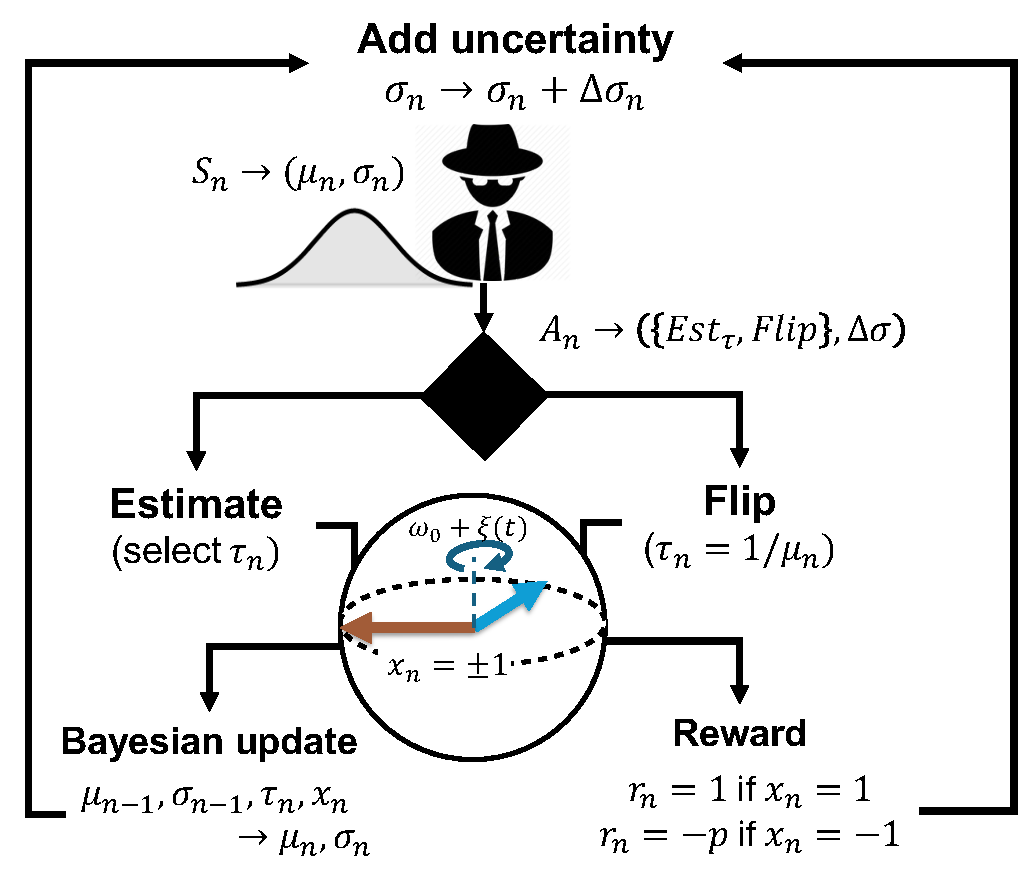
\includegraphics[width=\columnwidth]{scheme_RL.pdf}
    \caption{The scheme of the RL agent. The agent state is updated after each shot, and the agent decides between the estimation and the qubit operation. The agent is trained using the PPO algorithm.}
\end{figure}


\subsection{Dephasing}
Agent uncertainty or inaccuracy in the value of $\omega_n$ would result in over in under- or overrotation and lead to a decrease in the fidelity of qubit flip operation. According to agent best knowladge the $\pi$ pulse is realised by choosing the wainting time $\tau_n = \pi/\mu_n$, however the actual rotation angle is given by $\theta = \omega_n \tau_n = \pi \omega_n/\mu_n$, using which the average fidelity of the qubit flip yields
\begin{equation}
 F  = \langle P(1|\omega_n;\tau_n) \rangle_n = \frac{1}{2} - \frac{1}{2}\big\langle \cos(\pi \omega_n/\mu_{n-1})e^{-\pi\Gamma/\mu_{n-1}} \big\rangle_n,
\end{equation}
where $\langle \cdot \rangle$ stands for the average over the sufficiently many trials. 


Firstly, we consider the case in which there is no tracking, i.e. $\mu_{n-1} = \omega_0$, where $\omega_0$ is the average value of $\omega_n$. In such a case we have:
\begin{equation}
    F = \frac{1}{2} - \frac{1}{2} \exp\left(-\frac{\pi\Gamma}{\omega_0} - \frac{\pi^2 \sigma_\omega^2}{2\omega_0^2}\right).
\end{equation}

Next we model temporal correlations of the field by introducing a random variable $\Delta\omega_n = \omega_n - \omega_{n-1}$ and the estimation error through random variable $\delta \mu=\omega_n -\mu_n$. Both are indepdented of $\omega_n$ and modeled by Gaussian distribution of zero-average and variance $\sigma_{\Delta\omega}^2$ and $\sigma_{\delta\mu}^2$ respectively. For the field itself we use ergodic approximation, hence assume that the average over the trajectory of $\omega_n$ is equivalent to the average over fixed distribution $P(\omega)$. This corresponds to a situation, in which the data aquisition time is long enough for the field to explore the significant portion of its probability distribution []. With those assumptions the average infidelity is obtained by averaging over distribution of the $\omega$ and $\delta \mu$: 
\begin{equation}
    F  = \frac{1}{2} + \frac{1}{2} \chi
\end{equation}
where:
\begin{equation}
\chi \approx \left\langle \cos\left(\pi\frac{ \Delta \omega + \delta \mu}{\omega}\right)\exp(-\frac{\pi\Gamma}{\omega})  \right\rangle_{\omega, \Delta \omega, \delta \mu},
\end{equation}
where in the expression above, in the denominators we omitted $\delta \mu$ in comparison to $\omega$ assuming $\delta \mu, \Delta \omega \ll \omega$. With such a form it is straightforward to evaluate the average over the distribution of $\Delta \omega$ and $\delta \mu$:
\begin{equation}
    \chi = \left\langle \exp\left(-\frac{\pi^2(\sigma^2_{\delta \mu} + \sigma^2_{\Delta\omega})}{2\omega^2} - \frac{\pi\Gamma}{\omega} \right) \right\rangle_{\omega},
\end{equation}
however resulting average over $\omega$ is not straightforward to evaluate. Typically however one should consider the case in which the fluctuations takes place around a constant value $\omega_0$ that is much larger than the amplitude of the fluctuations, i.e. $\omega_0 \gg \sigma_{\Delta\omega}$, where $\omega \sim \mathcal(\omega_0, \sigma_{\Delta\omega})$. If additionally the $\chi$ is not too far from 1, i.e. dephasing is relatively weak we can expand the $\chi$ and use the fact that for the Gaussian distribution we have $\langle \omega^{-2} \rangle \sim \omega_0^{-2}$ and $\langle \omega^{-1} \rangle \sim \omega_0^{-1}$, which in leading order gives infidelity of spin flip
\begin{equation}
     1 - F \approx  \frac{\pi}{2\omega_0} \bigg(\Gamma + \pi\frac{\sigma^2_{\delta \mu} + \sigma^2_{\Delta\omega}}{2\omega_0}\bigg).
\end{equation}
Note that in the limit of no tracking  the estimation error is given by variation of the field around average value, i.e. $\sigma_{\delta \mu}^2 =  \sigma_{\omega}^2$, while the temproal variation no longer contributes to an error, i.e. $\sigma_{\Delta\omega} = 0$, which together allows to reconstruct Eq. (10).



\section{Metric, baselines and tests}

To evaluate the performance of the agent, we use the fidelity of the qubit flip, after the pi pulse. The fidelity is defined as
\begin{equation}
F = \frac{N_0}{N_\pi} 
\end{equation}
where $N_\pi =N_0 +N_1$ are the total number of flip attempts, while $N_0$ ($N_0$) are the number of successful (unsuccessful) flips. 

\section{Effect of temporal correlations}
Temporal correlations in the noise process, that extends behind a single shot time, can have a significant impact on the performance of the agent. 


Firstly, we consider the noise process that allows for tuning the correlation time. We use the Ornstein-Uhlenbeck process, that follows the diffusive equation
\begin{equation}
\text{d}\xi(t) = -\frac{1}{\tau_c} \xi(t) \text{d}t + \sqrt{\frac{2\sigma^2}{2\tau_c}}\text{d}W,
\end{equation}
where $\tau_c$ is the correlation time, $\sigma$ is the noise amplitude, and $dW$ is the Wiener incerement, such that $\int_0^t dW \sim \mathcal N(0,t)$. 



\section{1/f noise}
In this section we consider the 1/f noise, that is a common source of decoherence in solid-state qubits. We use the model of 1/f noise, that is a sum of many fluctuators with a Lorentzian spectrum, for which we use the Ornstein-Uhlenbeck process.






\end{document}



\end{document}